\documentclass{article}
\usepackage{graphicx}
\begin{document}
    \section*{Implementation}
        The implementation of this code was relatively straight forward given the structure, 
        we have to start by defining the initial conditions of two particles that we are then 
        going to model the position of the particle on the xy-plane, we start by setting initial
        mass scalars as well as position and momentum vectors. And then we calculated the momentary
        velocity at its position in order to determine the new position it will be at after a time step
        I had no large unexpected issues, however I did make a mistake when converting force to acceleration
        because I was accidentally treating force as differently for each particle which resulted in a bug that took me a while to find
        my debugging strategy started by reading over my code and the instructions and trying to find issues 
        then I selectively re-wrote lines of text which also didn't help, Finally I asked chat GPT to compare my code
        for individual problems against the description of the problem and that also proved useless cause it didn't find
        any errors. However on deeper thought I noticed force was the same on both particle one and two.
    \section*{Questions}
        \subsection*{1.}
        d84f3bae2366606c1bf60cce5e987d7aee7f1287
        \subsection*{2.}
        fp is declared in utilities.f90 and then 'use'd in every other fortran file
        \subsection*{3.}
        yes, orbit calls take\_step multiple times to fill the data into sol.dat so it makes sense to have it as its own
        module instead of just a subroutine
        \subsection*{4.}
        we would need to extend the lengths mass as well as the second index of position and momentum and then it would make our
        calculation for force more complicated, for a discrete number of particles you can still set the length of the arrays
        to be scalar values but for N particles you would have to declare them N length
        \subsection*{5.}
        3D space would be a greater challenge than adding more particles cause we would also have to change the way we graph our results
        but otherwise it would be about the same as adding more particles cause all that needs to be done is that the lengths of some of our arrays need tweaking
        and some of our equations as well.
        \subsection*{6.}
            \subsubsection*{Scenario 1:}
            \begin{figure}[h]  % 'h' tells LaTeX to place the figure 'here'
                \centering
                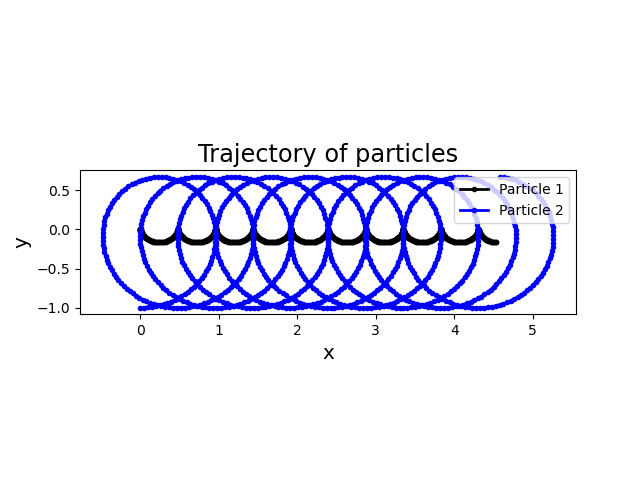
\includegraphics[width=0.5\textwidth]{Scenario_1.png}  % Adjust width as needed
                \label{fig:Scenario 1}
            \end{figure} 
            from scenario one with initial conditions: $m_1$ = 1, $m_2$ = 0.1  you can see that particle 2 has more of an effect on particle one due to its higher mass
            this will give the system more momentum as well, by printing the x and y coordinate of the 1000th time step we get the 
            momentum of the system is (0.1,0) which can be seen in the figure as it slowly moves to the right.
            
            \subsubsection*{Scenario 2:}
            \begin{figure}[h]  % 'h' tells LaTeX to place the figure 'here'
                \centering
                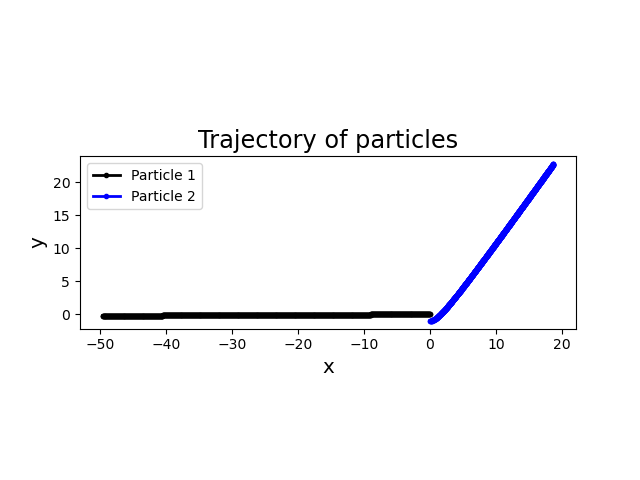
\includegraphics[width=0.5\textwidth]{Scenario_2.png}  % Adjust width as needed
                \label{fig:Scenario 2}
            \end{figure}
            From scenario two with initial conditions $p_1$ = (-1,0), $p_2$ = (1,0) we observe the particles instantly going in opposite directions
            and not orbiting each other at all
            % prompted chat GPT to learn how to make a new page cause the figure 3 was appearing above section
            \newpage

            \subsubsection*{Scenario 3:}
                \begin{figure}[h]  % 'h' tells LaTeX to place the figure 'here'
                    \centering
                    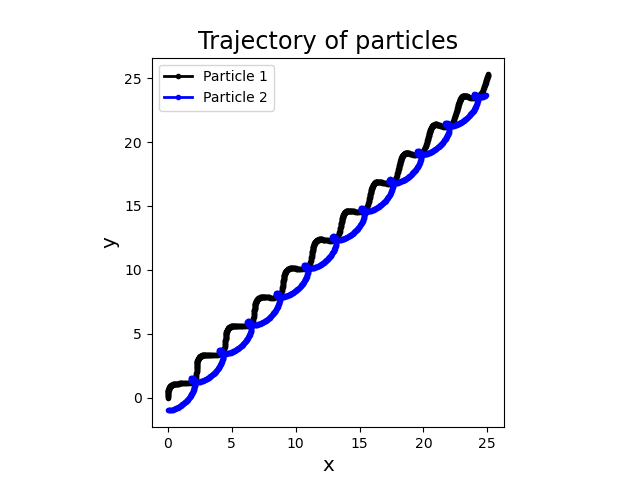
\includegraphics[width=0.5\textwidth]{Scenario_3.png}  % Adjust width as needed
                    \label{fig:Scenario 3}
                \end{figure}
                From scenario 3 with initial conditions $m_1$ = 1, $m_2$ = 1, $p_1$ = (0,1), $p_2$ = (1,0) we observe the particles slowly orbiting each other on the line y=x
                computing the momentum of the system gives us (1,1) which explains the very even, consistent nature of the graph





        \subsection*{7.}
        "-Wall -Wextra -ffree-line-length-none -fPIC -g -fcheck=all -fbacktrace", the first two flags starting with W warn you of errors
        the the 3rd flag isn't quite clear from the reading, prompted chatGPT with an ELI5 prompt the response informed me that this flag 
        allows for infinitely long lines of code. -fPIC also not clear from LLM response it seems to either enable the linking of your compilation 
        files or is just an effect of modernization of an old language. -g generates extra debugging info. -fcheck=all protects us from index out of bounds errors
        and -fbacktrace is also for debugging and can help to find the point of a crash
        \subsection*{8.}
        the assignment was using ODEs to solve a 2 body orbit problem and plot the coordinates of two particles onto an xy-plane
        our results show how well we can see the effect of a light body on a heavy body as the ripple in the path of particle one is pretty clear
        %used LLM output to help import a picture into latex
        \begin{figure}[h]  % 'h' tells LaTeX to place the figure 'here'
            \centering
            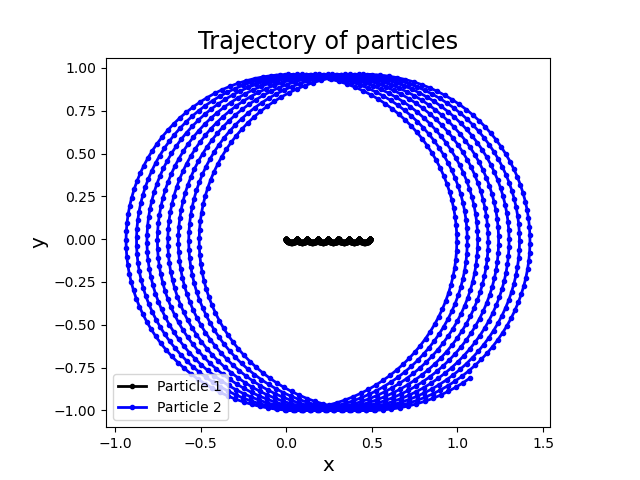
\includegraphics[width=0.5\textwidth]{result_graph.png}  % Adjust width as needed
            \caption{output from program}
            \label{fig:example}
        \end{figure}


\end{document}